\documentclass[letterpaper,11pt]{article}
\oddsidemargin -1.0cm \textwidth 17.5cm

\usepackage[utf8]{inputenc}
\usepackage[activeacute,spanish, es-lcroman]{babel}
\decimalpoint
\usepackage{amsfonts,setspace}
\usepackage{amsmath}
\usepackage{amssymb, amsmath, amsthm}
\usepackage{comment}
\usepackage{float}
\usepackage{amssymb}
\usepackage{dsfont}
\usepackage{anysize}
\usepackage{multicol}
\usepackage{enumerate}
\usepackage{graphicx}
\usepackage[left=1.5cm,top=2cm,right=1.5cm, bottom=1.7cm]{geometry}
\setlength\headheight{1.5em} 
\usepackage{fancyhdr}
\usepackage{multicol}
\usepackage{hyperref}
\usepackage{wrapfig}
\usepackage{subcaption}
\usepackage{siunitx}
\usepackage{cancel}
\usepackage{mdwlist}
\usepackage{svg}
\pagestyle{fancy}
\fancyhf{}
\renewcommand{\labelenumi}{\normalsize\bfseries P\arabic{enumi}.}
\renewcommand{\labelenumii}{\normalsize\bfseries (\alph{enumii})}
\renewcommand{\labelenumiii}{\normalsize\bfseries \roman{enumiii})}


\begin{document}

\fancyhead[L]{\itshape{Facultad de Ciencias F\'isicas y Matem\'aticas}}
\fancyhead[R]{\itshape{Universidad de Chile}}
\rfoot[]{pág. \thepage}

\begin{minipage}{11.5cm}
    \begin{flushleft}
        \hspace*{-0.6cm}\textbf{FI1000-1 Introducción a la Física Clásica}\\
        \hspace*{-0.6cm}\textbf{Profesor:} Ignacio Bordeu\\
        \hspace*{-0.6cm}\textbf{Auxiliares:} Alejandro Cartes \& Simón Yáñez\\
        \hspace*{-0.6cm}\textbf{Ayudante:} Javier Cubillos\\
    \end{flushleft}
\end{minipage}

\begin{picture}(2,3)
    \put(366, 10){
\includegraphics[scale=0.9]{2020-1/Imágenes/logo/dfi-fcfm.pdf}}
\end{picture}

\begin{center}
	\LARGE\textbf{Auxiliar \#12}\\
	\Large{Centro de Masa}
\end{center}

\vspace{-1cm}
\begin{enumerate}\setlength{\itemsep}{0.4cm}

\item[]

\item
\begin{enumerate}
    \item Determine el centro de masa del sistema mostrado en la figura (1) utilizando el mismo sistema de referencia presentado
    
    \item Los objetos de la figura (2) están hechos de un alambre uniforme doblado. Determine la posición del centro de masa de cada uno

    \begin{figure}[H]
        \centering
        \begin{subfigure}[t]{0.25\textwidth}
            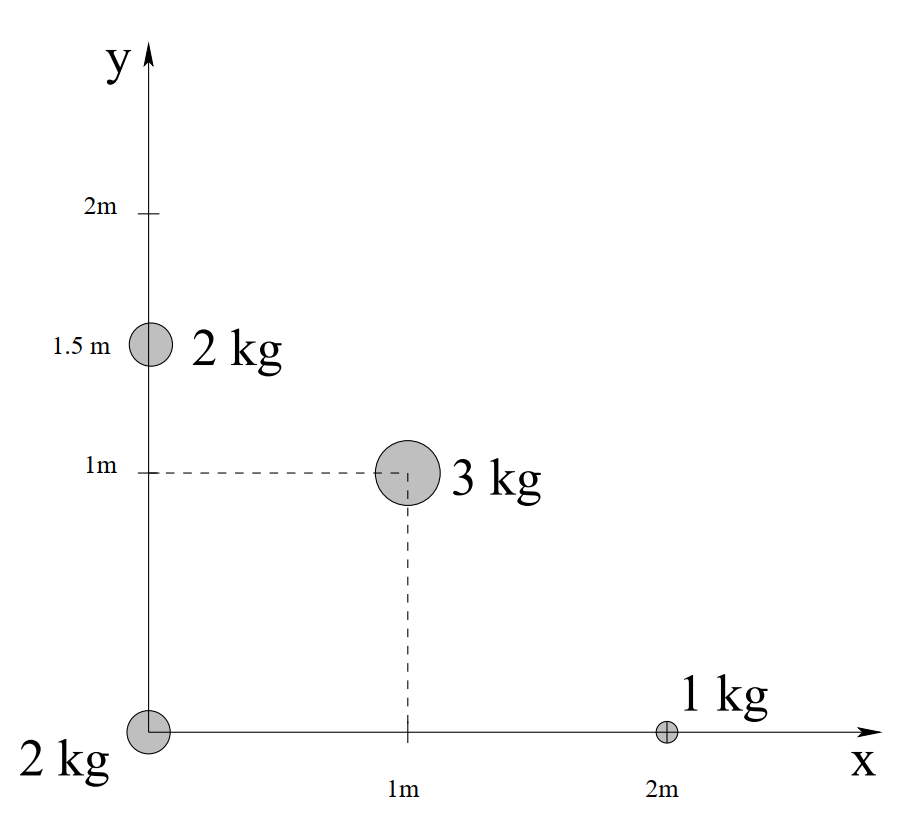
\includegraphics[width=1\linewidth]{2023-1/img/aux_12/axis.png}
            \caption*{1) Sistema}
        \end{subfigure}
        \hspace{3em}
        \begin{subfigure}[t]{0.6\textwidth}
            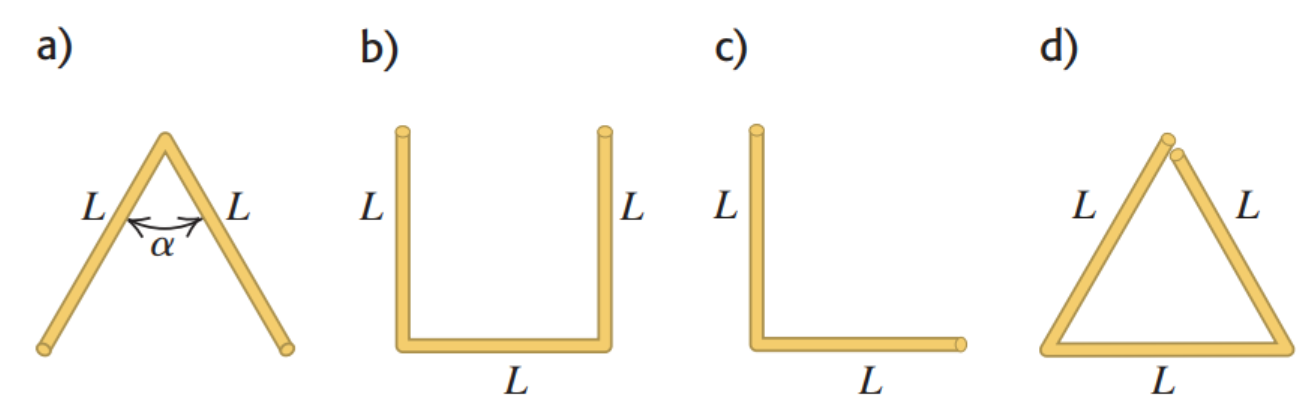
\includegraphics[width=1\linewidth]{2023-1/img/aux_12/alambres.png}
            \caption*{2) Alambres}
        \end{subfigure}
    \end{figure}
\end{enumerate}

\item Un perro de masa $m$ está sentado en un extremo de un bote de masa $M$ y largo $L$ que se ubica junto a un muelle, tal como se muestra en la figura. El perro decide ir por unas deliciosas galletas perrunas que lo esperan en su casa, por lo que camina hasta el otro extremo del bote para luego salir por el muelle. Lamentablemente, cuando el perrito llega, se da cuenta que se encuentra a una distancia $D$ del muelle.

\begin{multicols}{2}
    \begin{enumerate}
        \item Determine $D$ en términos de $m$, $M$ y $L$. Asuma que el bote es completamente simétrico
        
        \item Si $D < L/2$, el perrito puede saltar para llegar al muelle, en caso contrario tendrá que nadar. Determine la razón $m/M$ límite para la cual el perrito no tenga que llegar mojado por sus galletas.
    \end{enumerate}
    
    \columnbreak
    
    \begin{figure}[H]
        \centering
        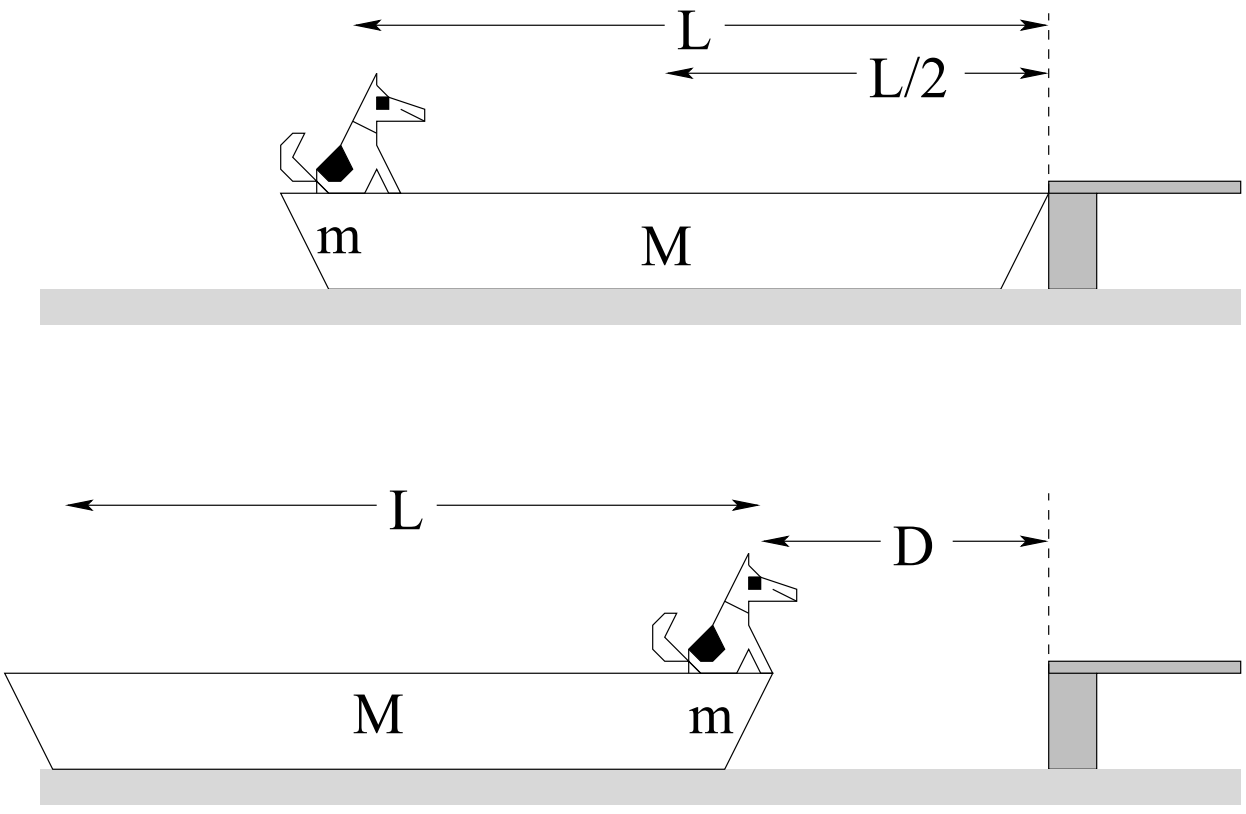
\includegraphics[width = 0.73\linewidth]{2022-1/img/aux11/perrito.PNG}
    \end{figure}
    
\end{multicols}

\begin{multicols}{2}
\item Se lanza un proyectil con una rapidez inicial $v_0$, formando un ángulo de $\theta_0$ con respecto a la horizontal. En el punto más alto de su vuelo, el proyectil explota rompiéndose en dos partes, una de las cuales tiene el doble de masa que la otra. Los dos fragmentos salen inicialmente despedidos en la dirección horizontal (como se indica en la figura), y aterrizan simultáneamente. Si el fragmento más ligero aterriza a una distancia $L$ del punto de lanzamiento, determine la posición $\ell$ donde aterrizará el otro fragmento.

\columnbreak

\begin{figure}[H]
    \centering
    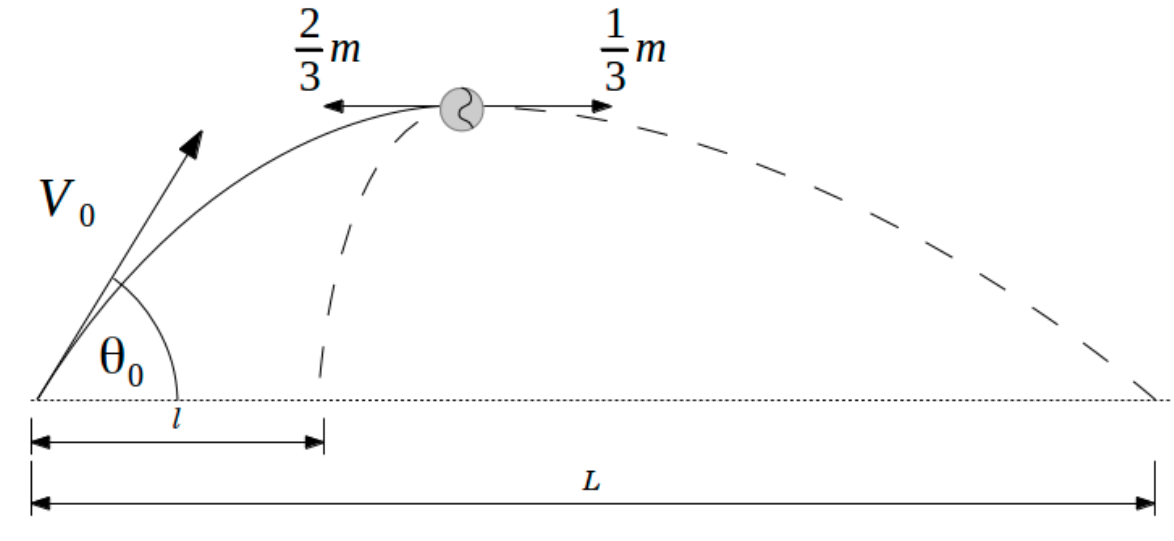
\includegraphics[width=0.9\linewidth]{2021-2/img/aux11/proyectil.PNG}
\end{figure}

\end{multicols}

% Para imágenes vectoriales -> el texto tiene que estar en LaTeX
% \begin{figure}[htbp]
%   \centering
%   \svgpath{../Imagenes/ejercicios}  -> .. irse pa'trás 
%   \includesvg{ej5.svg}
% \end{figure}

\end{enumerate}
\end{document}
